Un leñador corta una pieza en forma de cuña $W$ de un árbol cilíndrico de radio $r$
obtenido de hacer dos cortes de sierra en el centro del árbol, uno horizontal
y otro en un ángulo $\theta$. Calcula el volumen de la cuña $W$ usando el 
principio de Cavalieri. 
Véase la figura
\begin{figure}[H]
    \begin{center}
        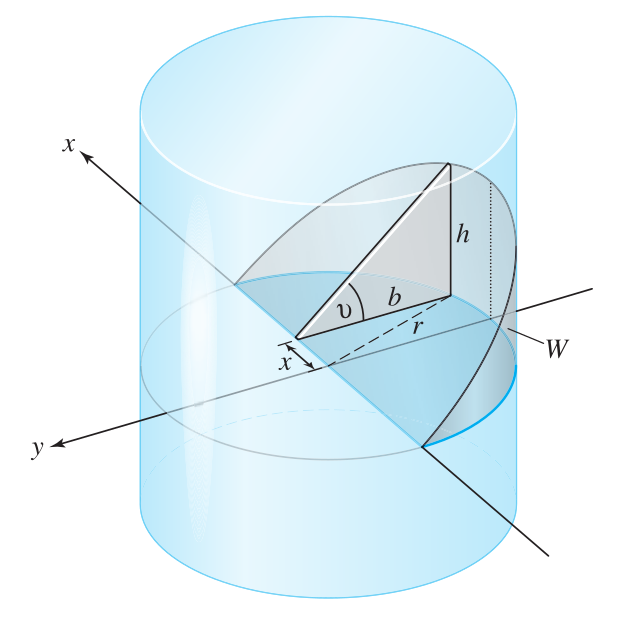
\includegraphics[width=0.3\textwidth]{img/Ej2/ej7.png}
    \end{center}
\end{figure}
\begin{solution}
    Como lo muestra la figura, podemos pensar en las secciones triangulares paralelas que dependen
    de $x$, que es la distancia de la punta de la sección al centr del círculo.
    Por otro lado, podemos observar un triángulo rectángulo formado por los de 
    longitud $x$, $r$ y $b$. Por lo tanto 
    \[
        b=\sqrt{r^2-x^2}.
    \]
    Así que podemos ver, 
    por la definición de tangente, que $h=b\tan \theta=\sqrt{r^2-x^2}\tan \theta$.
    Entonces el área de cada triángulo es 
    \[
        T(x)
        =
        \frac{1}{2} 
        \left(\sqrt{r^2-x^2}\right)
        \left( \sqrt{r^2-x^2}\tan \theta \right).
    \]
    De esta manera, por el principio de Cavalieri el volumen de la cuña es 
    \begin{align*}
        \mathrm{vol}(W)
        &=
        \int_{-r}^{r}
        T(x)
        \, dx
        =
        \int_{-r}^{r}
        \frac{\tan\theta}{2} (r^2-x^2)
        \, dx
        \\
        &=
        \tan\theta
        \int_{0}^{r}
        (r^2-x^2)
        \, dx,\quad\text{por la paridad del integrando,}\\
        &=
        \tan \theta
        \int_{0}^r
        r^2\, dx
        -\tan\theta
        \int_0^r
        x^2\, dx\\
        &=
        r^3\tan\theta-\tan\theta \frac{r^3}{3} = \frac{2 r^3 \tan \theta}{3}.
    \end{align*}
\end{solution}
